\documentclass{article}


\usepackage{arxiv}

\usepackage[utf8]{inputenc} % allow utf-8 input
\usepackage[T1]{fontenc}    % use 8-bit T1 fonts
\usepackage{hyperref}       % hyperlinks
\usepackage{url}            % simple URL typesetting
\usepackage{booktabs}       % professional-quality tables
\usepackage{amsfonts}       % blackboard math symbols
\usepackage{nicefrac}       % compact symbols for 1/2, etc.
\usepackage{microtype}      % microtypography
\usepackage{lipsum}
\usepackage{graphicx}
\graphicspath{ {./images/} }


\title{Attention Phrenology: A spatial classification of attention heads}


\author{
 Giles Edkins \\
  Alignment Jam \#4 \\
  \texttt{edkins@gmail.com} \\
   \And
 Keira Wiechecki \\
  Alignment Jam \#4 \\
  Department of Biology \\
  New York University \\
  \texttt{kaw504@nyu.edu} \\
}

\begin{document}
\maketitle
\begin{abstract}
Even with the same architecture, input, and tokens, the internal parameters of two language models can diverge substantially. However, they can nonetheless be made to converge on the same result. We attempt to determine whether heads with similar functions can be identified in different models. We present what we believe to be a novel method of language model interpretability analysis taking inspiration from biological imaging analysis.

\end{abstract}


% keywords can be removed
\keywords{Mechanistic Interpretability \and ML Safety \and Transformers}


\section{Introduction}


\section{Methods}
We trained 9 toy language models on [corpus]

We extracted weights from each head from each model in response to 1024 prompts. We used an autoencoder to compress the weights for each token pair into between 2 and 64 embedding dimensions. We used Akaike Information Criterion to select the most informative number of embedding dimensions.

\subsection{Giles Methods}
\subsubsection{Model Architecture}

9 models were trained. Each model was constructed using the **TransformerLens library. Each has the same architecture:
\begin{itemize}
	\item A single layer
	\item 8 Heads
	\item A context window of 16 tokens
	\item A model dimensionality of 256
	\item A head dimensionality of 64
	\item An MLP dimensionality of 2048
	\item A solu activation function
	\item The tokenizer taken from GPT-2
\end{itemize}

\subsubsection{Training}
Each model was trained for 4 epochs, with a sample of 30,000 datapoints (each 16 tokens long) taken from the **Brown corpus. An **AdamW optimizer was used, and a cross-entropy loss function.

\subsubsection{Attention weight extraction}
A sample of 1024 datapoints (each 16 tokens long) was taken from the Brown corpus. Each datapoint was fed through each model to calculate the logits, which were discarded - instead, we captured the attention pattern of each attention head. This was saved as a big CSV file.

\subsubsection{Head-distance matrix}
For each head of each model (72 total), we took all the attenion values and treated them as one long vector. Then we took the Euclidean distance between pairs of these vectors, to generate a 72x72 matrix.

\subsubsection{UMAP, TSNE and PCA visualizations}
We ran a 2-component Principal Component Analysis, UMAP and TSNE where the datapoints corresponded to the model-heads, and the features corresponded to attention weights on the different prompts. The projected components are shown, together with projections for 3 artificial points:

\begin{itemize}
	\item Each token only attending to itself
	\item Each token attending to all previous tokens equally
	\item Each token attending to itself and the previous token
\end{itemize}

\subsubsection{PCA components}
We ran a Principal Component Analysis where the datapoints corresponded to the model-heads, and the features corresponded to attention weights on the different prompts. The first 5 principal components, and the first 8 prompts, are shown.

\subsubsection{How much each token attends to the first token}
As a follow-up, we plotted a PCA projection of the attentions of various words in various prompts, against the first word only.

\subsubsection{Head knockout}
Here, further information was gathered from the models. In particular, we used the TransformerLens hook feature to erase the output from one of the heads on the given model, to investigate the effect of that head on the output. This allows, for a given prompt, producing a scatterplot of each token: the x-axis is the original logit values from the model, and the y-axis shows the logits when the head is knocked out.

The idea is that tokens above the diagonal are "suppressed" by the given head, and tokens below the diagonal are "promoted" by that head.

As a further investigation, we produced similar plots for each of the model-heads in one of the clusters, to see if they promote/suppress similar tokens.

\subsubsection{Head knockout with multiple prompts}
Finally, we took a selection of 64 prompts from the corpus and used the difference in probabilities (not logits) as a vector. Then we applied PCA dimensionality reduction to this and colored them according to the original clusters. The idea was to see whether clustering in the attention weights corresponds to clustering in the promoted/suppressed token space.

\section{Results}

\begin{figure}
	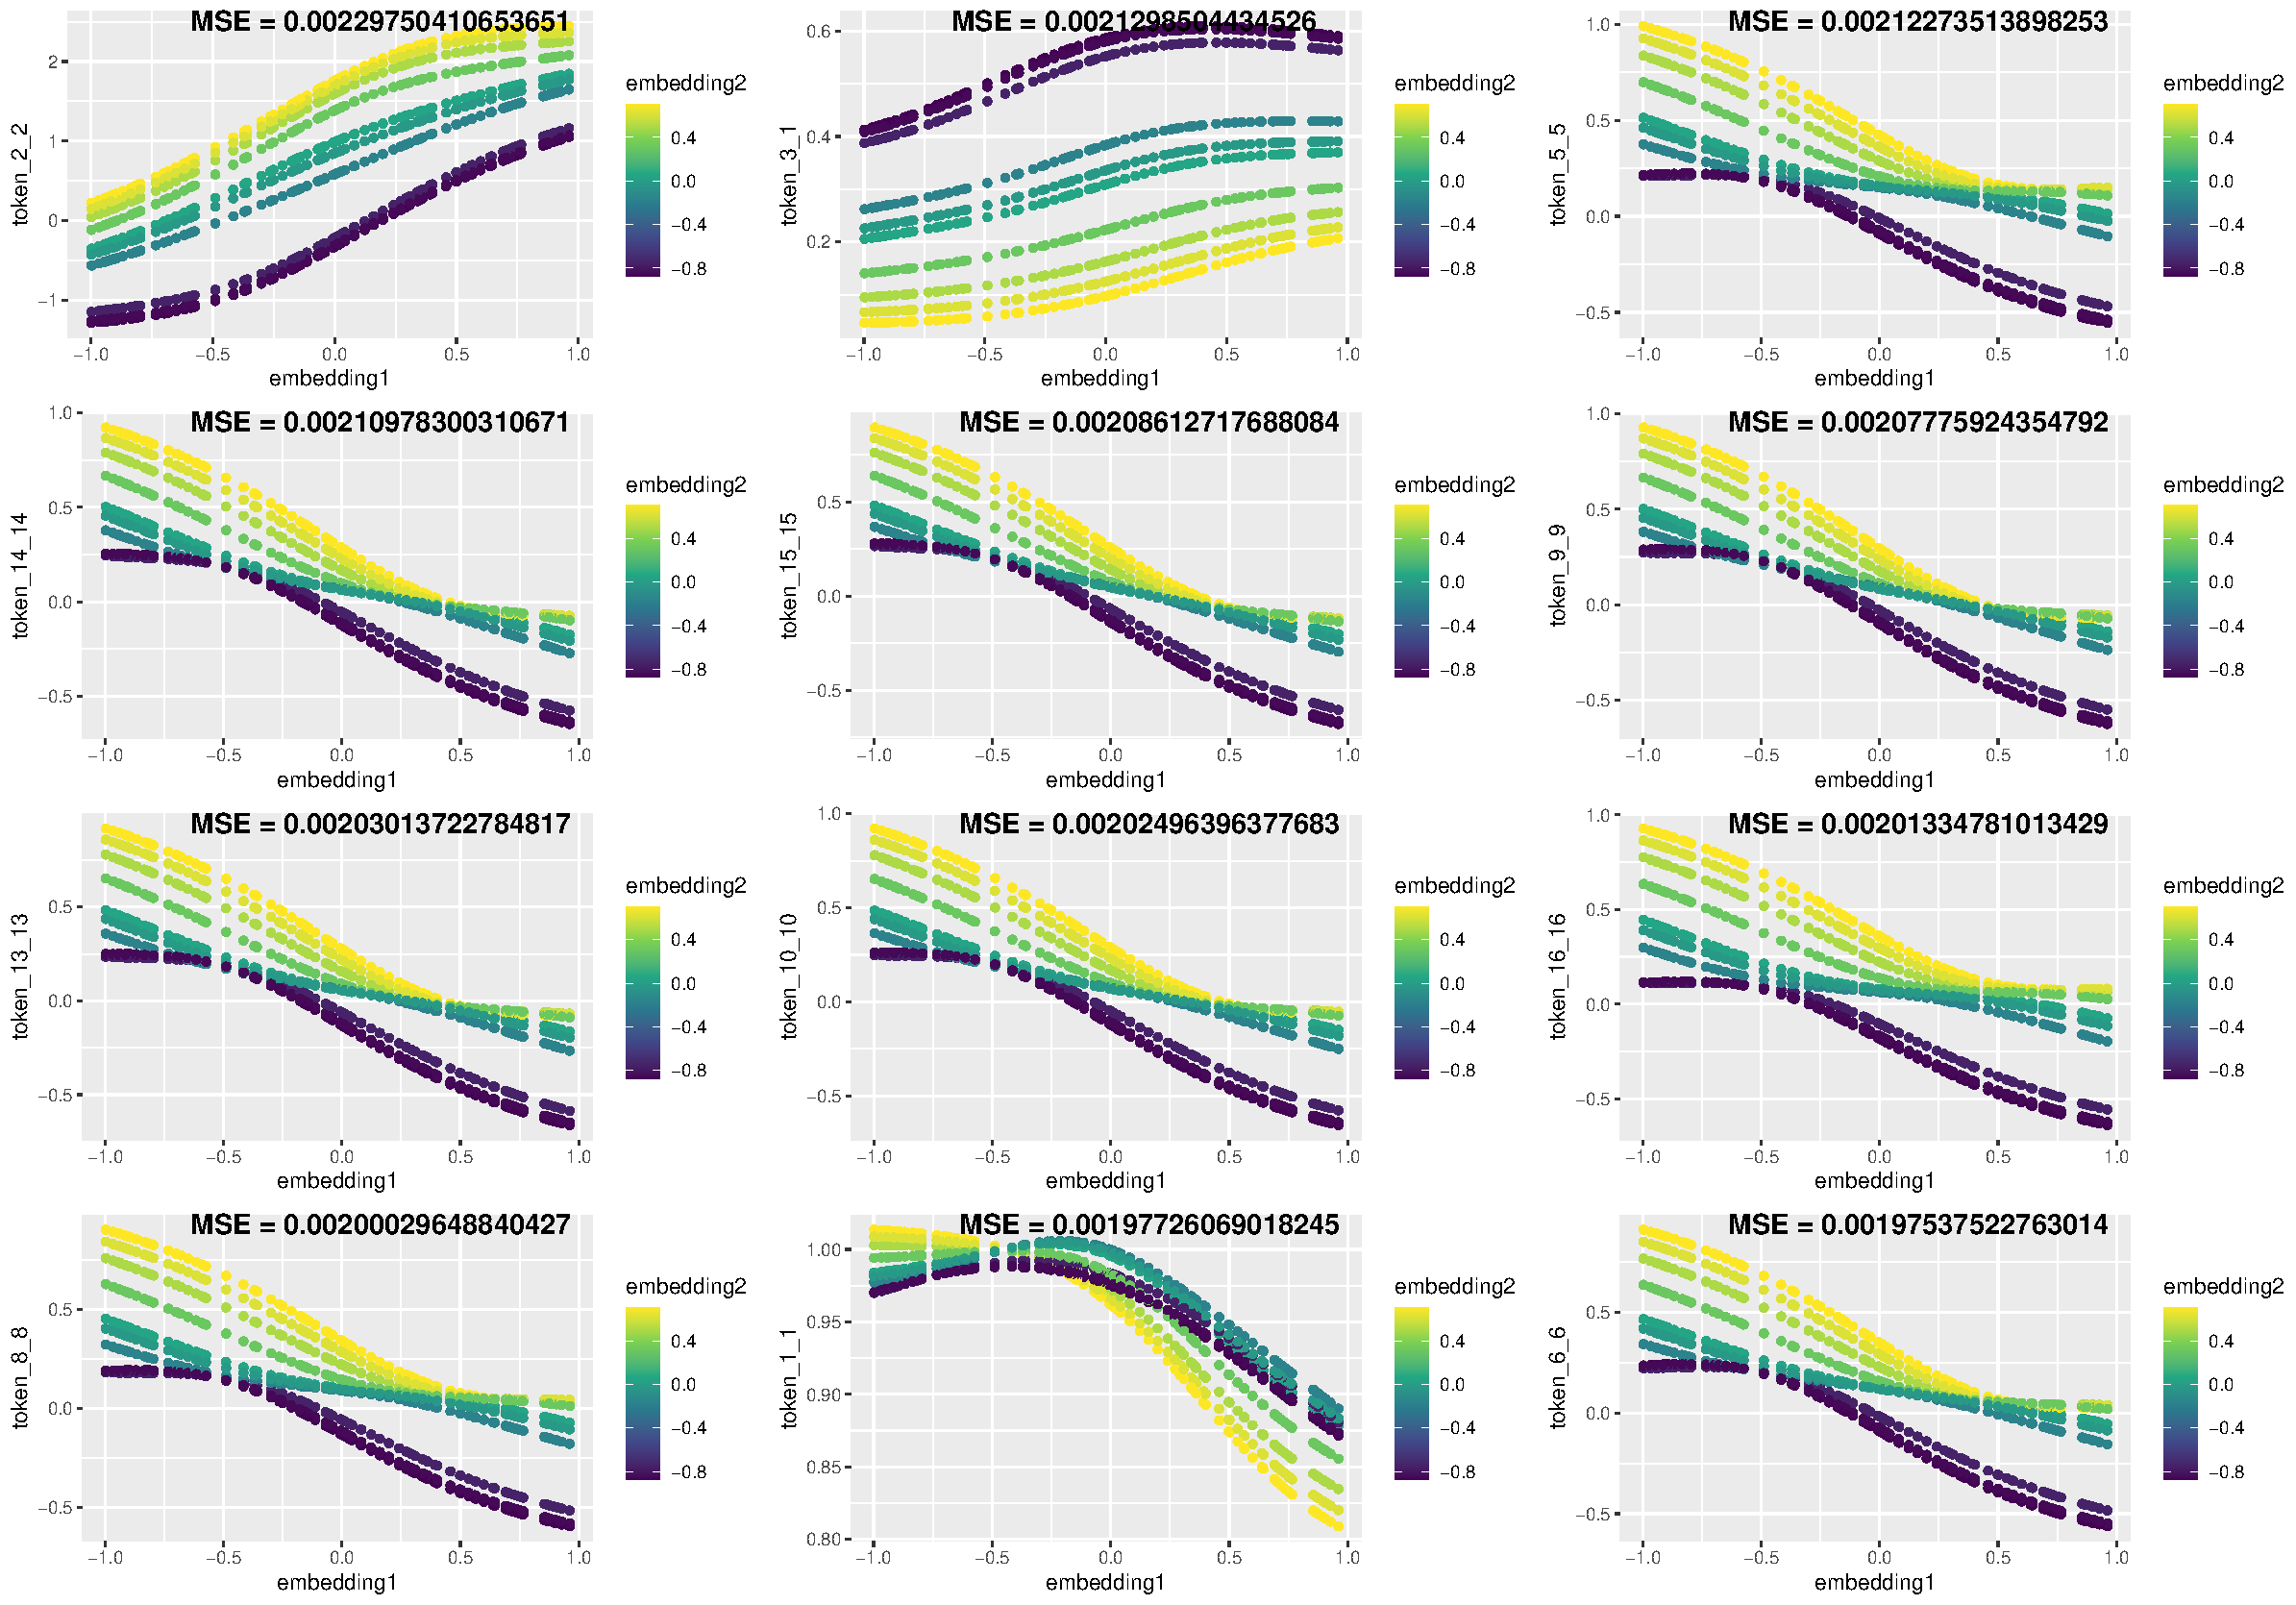
\includegraphics[width=\textwidth]{figs/top.embeddings.pdf}
	\caption{Decoded token pair weights generated by embedding value pairs. MSE values were calculated based on how well the autoencoder recovered the input when the indicated token pair was randomized in the input.}
	\label{}
\end{figure}

\begin{figure}
	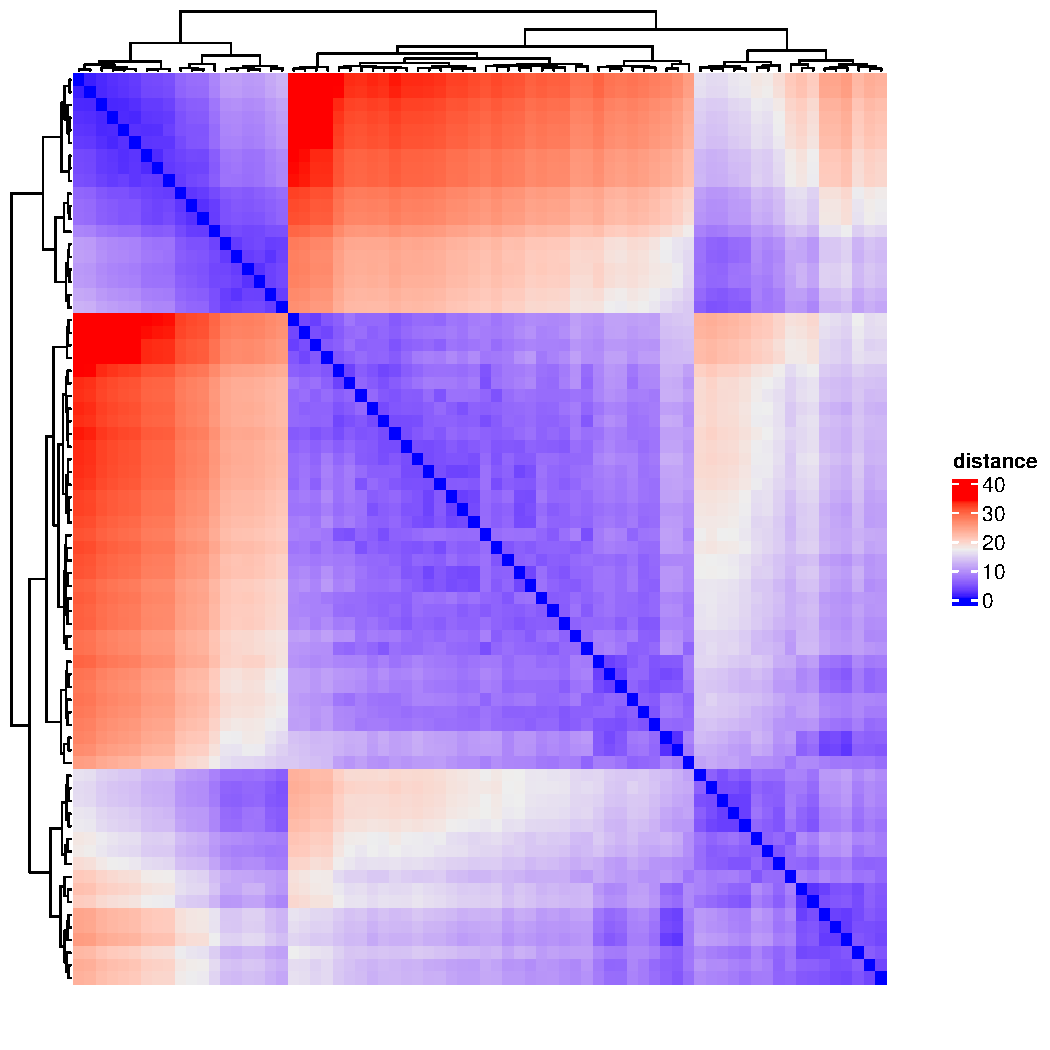
\includegraphics[width=\textwidth]{figs/dist.pdf}
	\caption{Pairwise euclidean distance between attention head embeddings.}
	\label{}
\end{figure}

\begin{figure}
	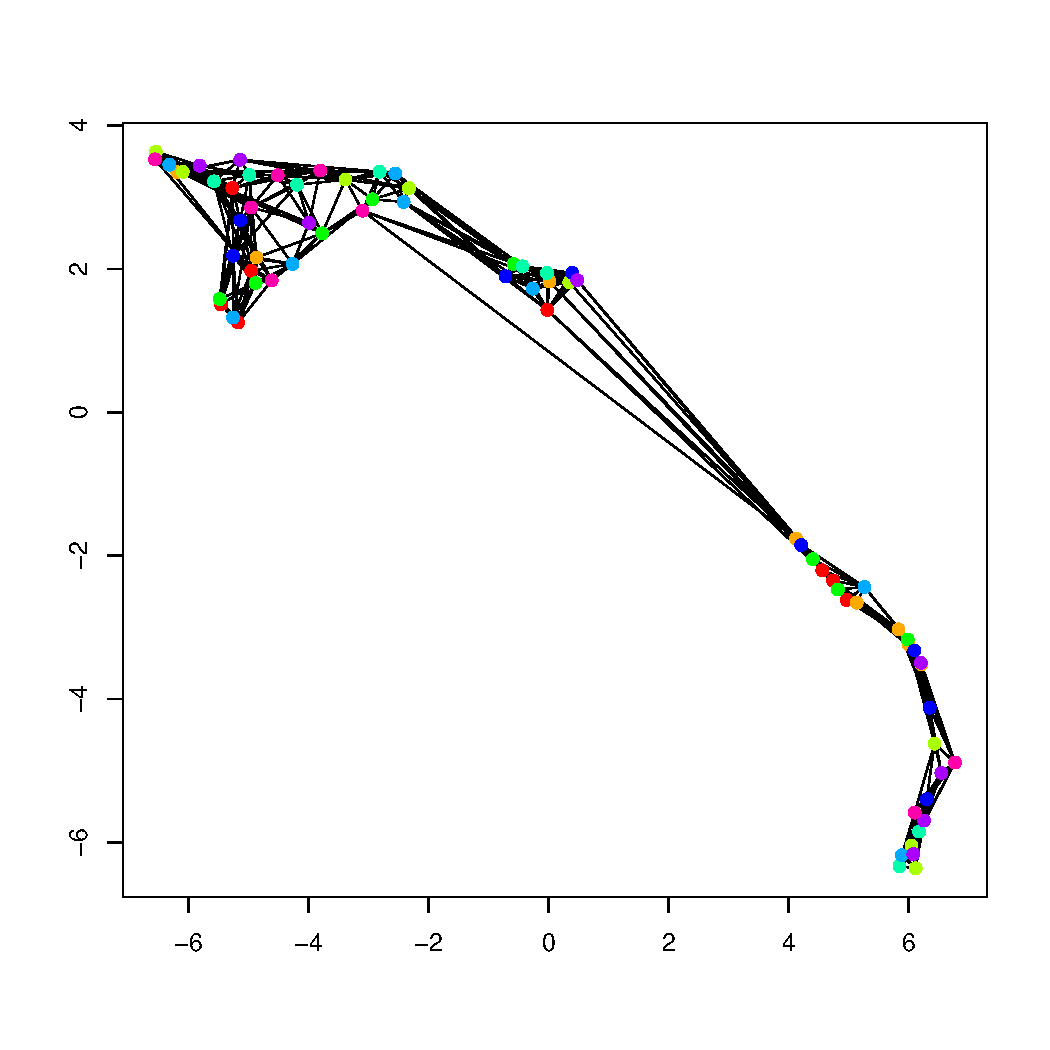
\includegraphics[width=\textwidth]{figs/knn.pdf}
	\caption{9-nearest neighbors graph of attention head embeddings. Heads are color coded by model.}
	\label{}
\end{figure}

\begin{figure}
	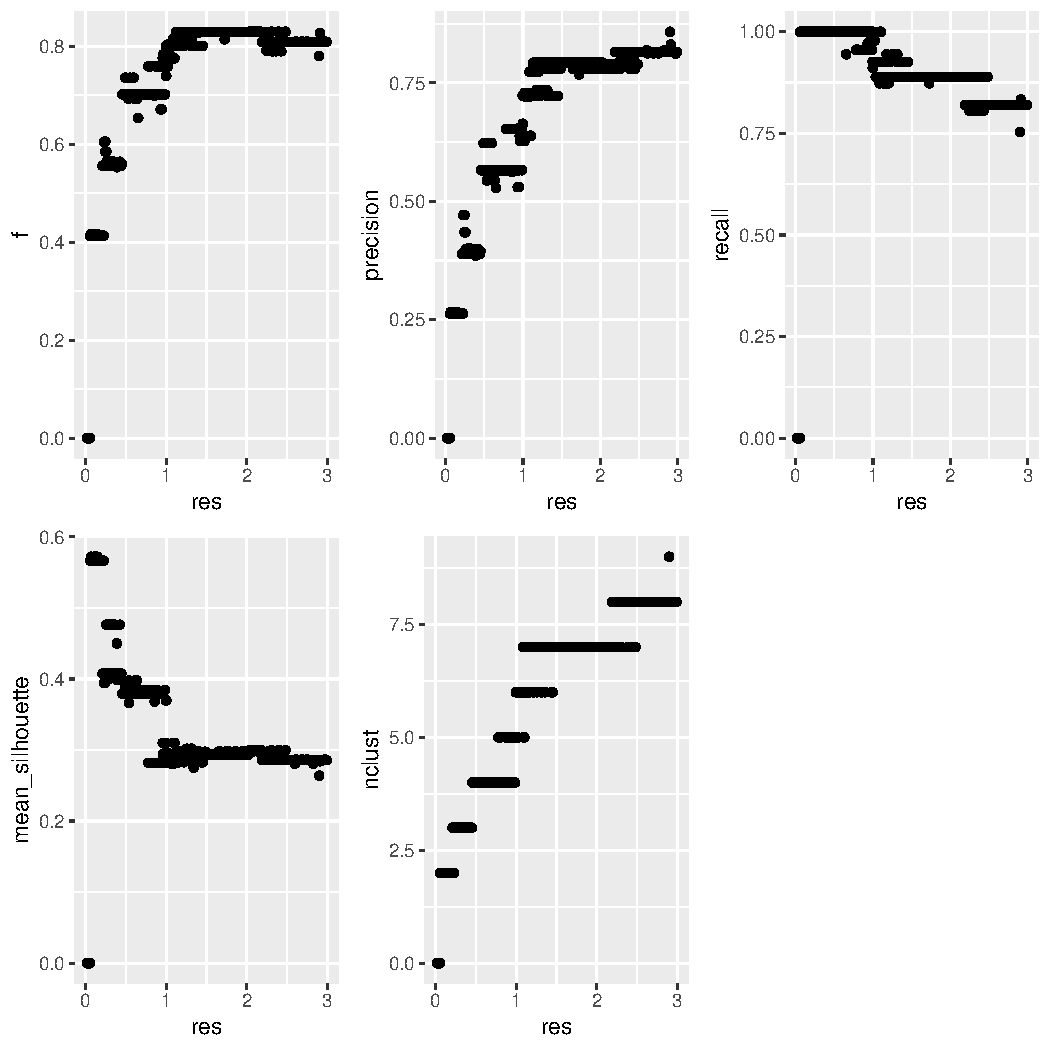
\includegraphics[width=\textwidth]{figs/optimization.pdf}
	\caption{Optimization of \gamma selection.}
	\label{}
\end{figure}

\begin{figure}
	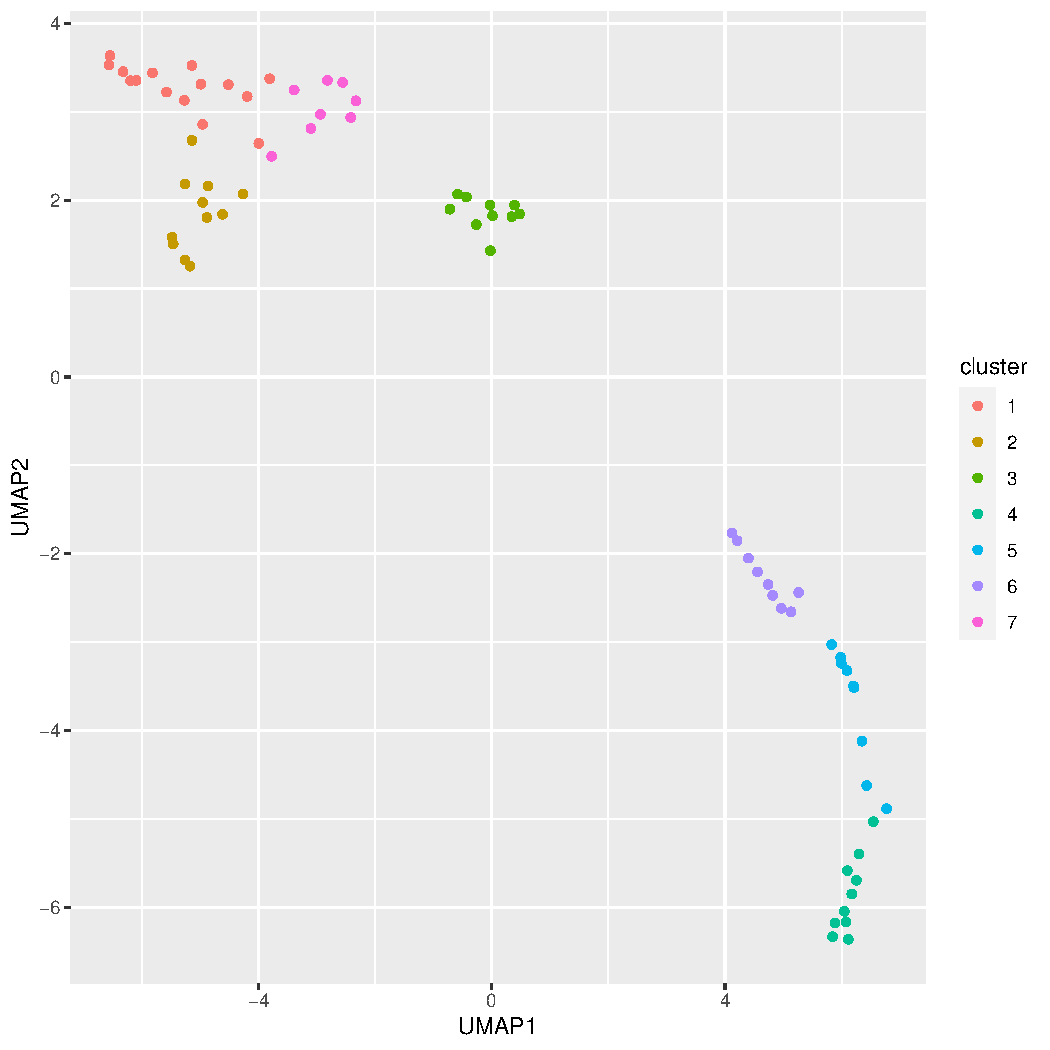
\includegraphics[width=\textwidth]{figs/encoding.pdf}
	\caption{Optimal clustering at \gamma = 2.16.}
	\label{}
\end{figure}

\begin{figure}
	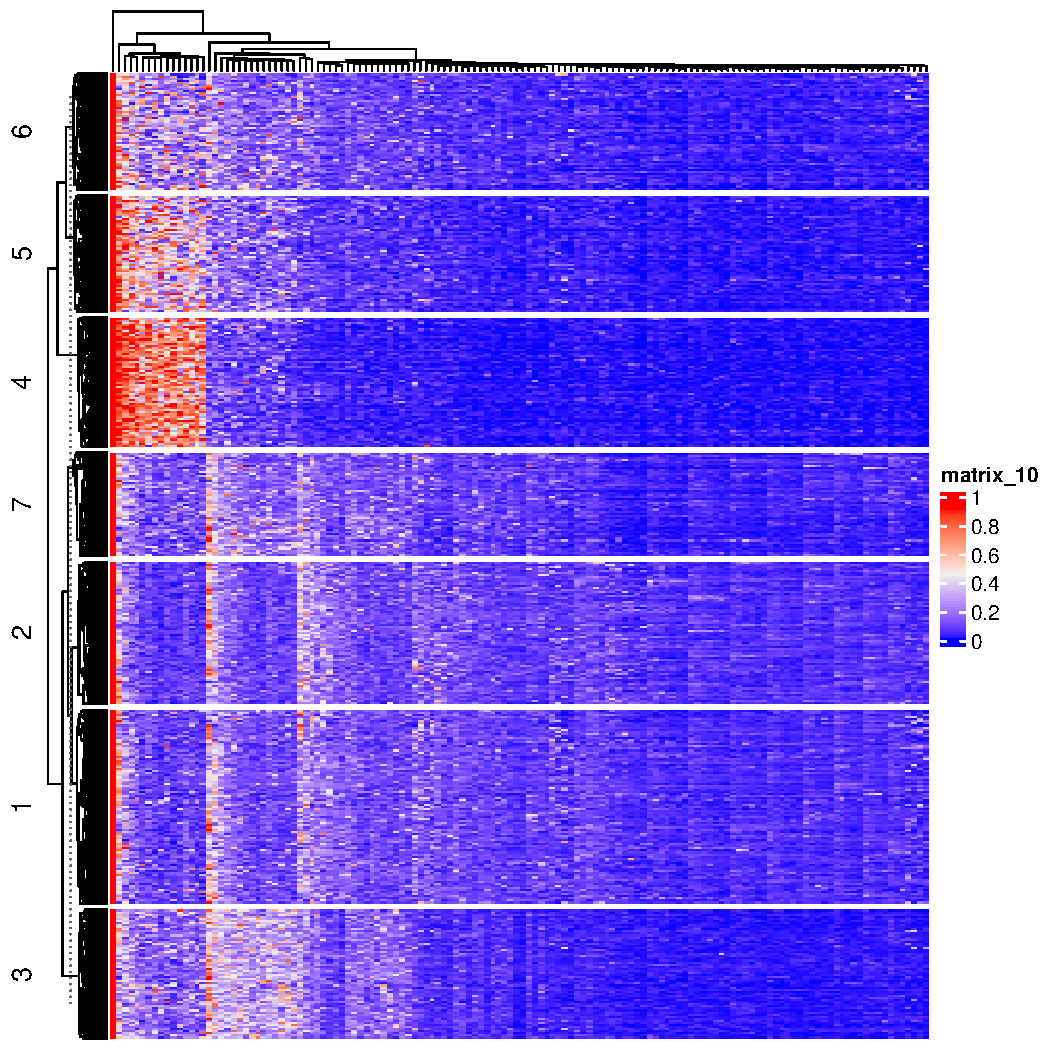
\includegraphics[width=\textwidth]{figs/clusthm.pdf}
	\caption{Token pair weights by cluster.}
	\label{}
\end{figure}

\subsection{Giles Results}

In \ref{fig:head-distance-matrix} we see, obviously, that each head is identical to itself (the diagonal). We see some heads that stand out as being generally different, but similar to each other (the horizontal and vertical yellow lines). These roughly correspond to heads that mostly have each token attending to itself. Some other heads are a little closer or further than average but none are identical in their behavior.

\begin{figure}
    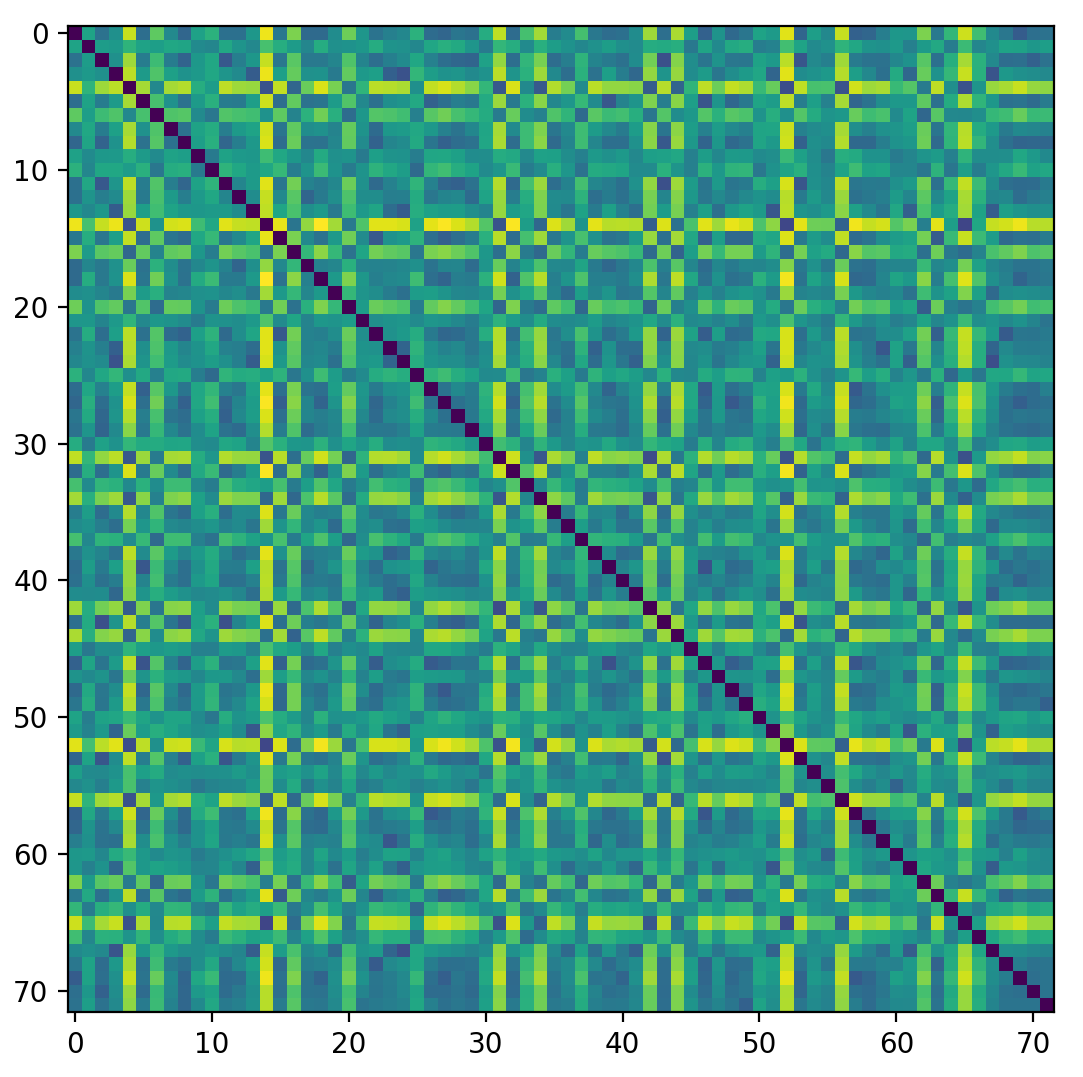
\includegraphics[width=\textwidth]{images/head-distance-matrix.png}
    \caption{Pairwise euclidean distance between attention head embeddings, arranged in the original order.}
    \label{fig:head-distance-matrix}
\end{figure}

In \ref{fig:umap-tsne-pca} we see the black dot (corresponding to attending to everything equally) is central to one of the clusters of heads. The two grey dots (dark grey corresponding to attending to the current token, and light grey corresponding to attending to the current and previous tokens) are less central but still fairly close to real head clusters.

\begin{figure}
    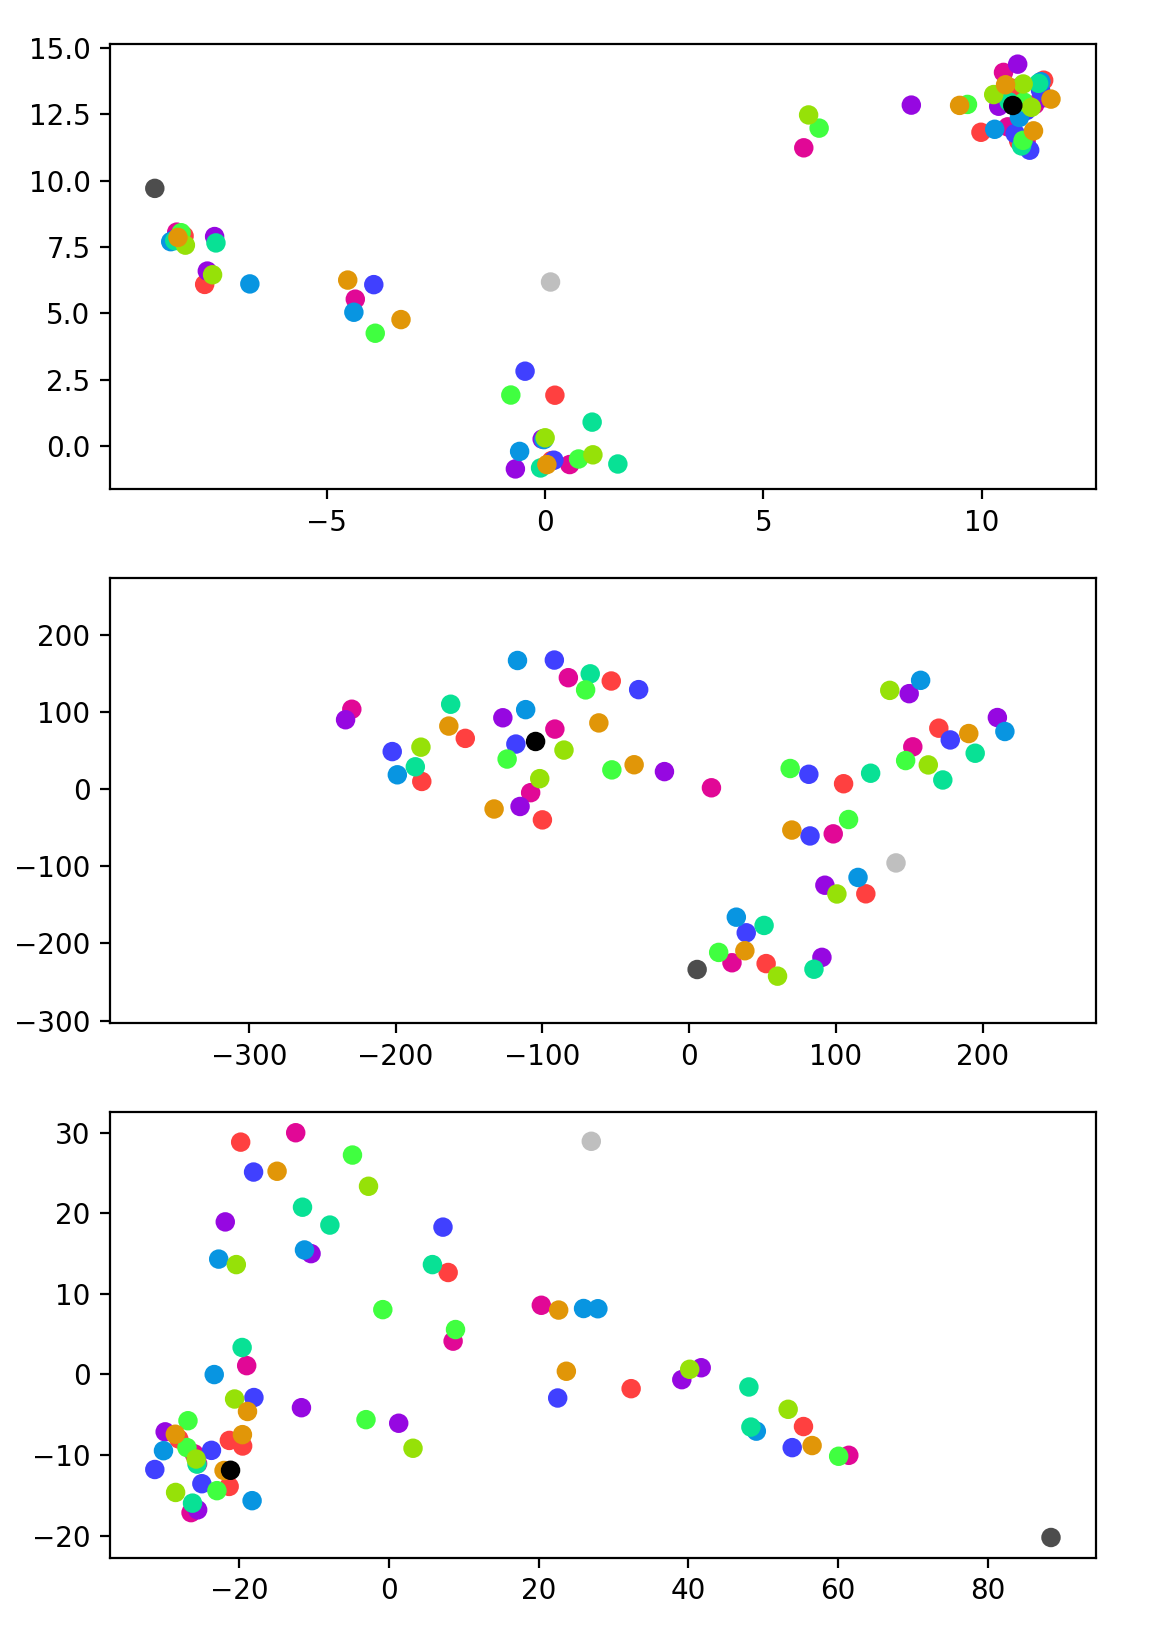
\includegraphics[width=\textwidth]{images/umap-tsne-pca.png}
    \caption{UMAP, TSNE, PCA dimension reductions of attention head embeddings together with artificial points in grey.}
    \label{fig:umap-tsne-pca}
\end{figure}

In \ref{fig:pca-components} we see the first principal component has entries along each of the diagonals, corresponding to attending to the current token.

The second principal component corresponds (roughly) to attendig to the previous token, although there are some wiggles.

The remaining principal components exhibit different behaviour for each prompt, and warrant further investigation. The third principal component is shown in \ref{fig:pca-component-2}. This shows one sign for the first column (attending to the first token in the sequence) and the opposite sign for the remaining tokens. Furthermore, the sign is positive (red) for common "stop-words" such as "the", "of" and "and" and negative (blue) for more semantically meaningful words.

This effect is explored further in \ref{fig:attention-to-first-token}, where we see how much each token attends to the first token, across all model-heads, but reduced to 2 dimensions with PCA. This shows a clear cluster of capitalized words up the top-right, and stop-words towards the lower-right of the main cluster.

\begin{figure}
    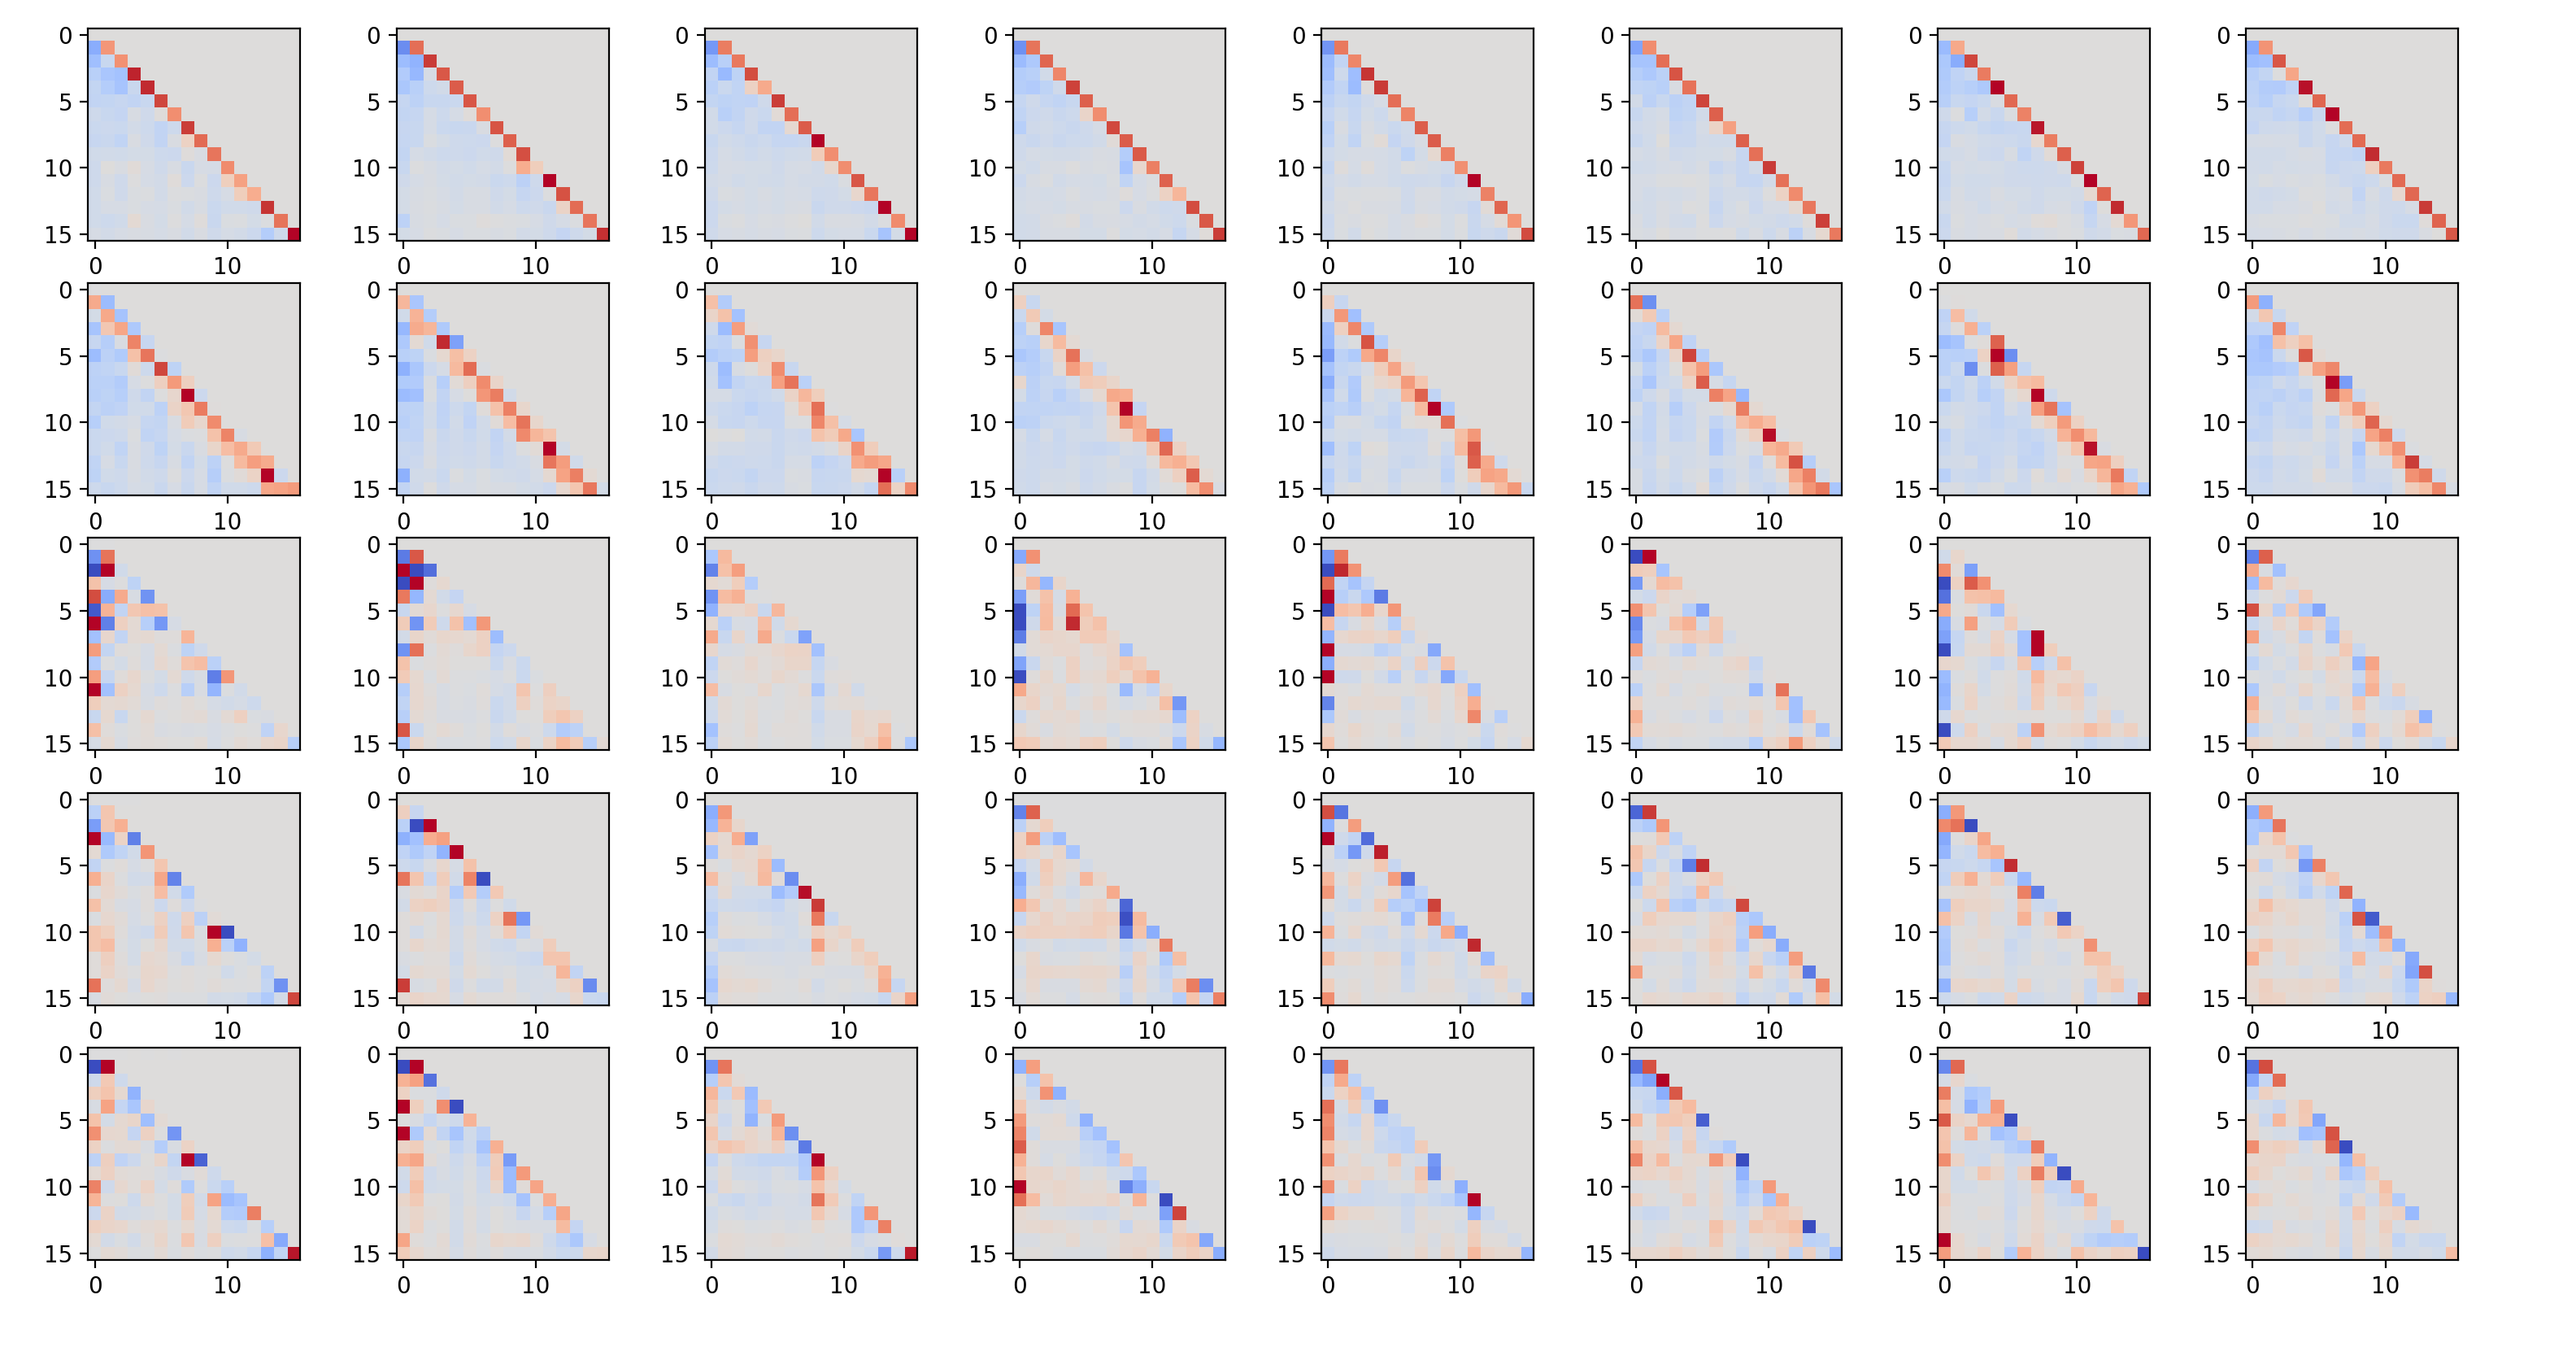
\includegraphics[width=\textwidth]{images/pca-components.png}
    \caption{PCA components of attention head embedding}
    \label{fig:pca-components}
\end{figure}

\begin{figure}
    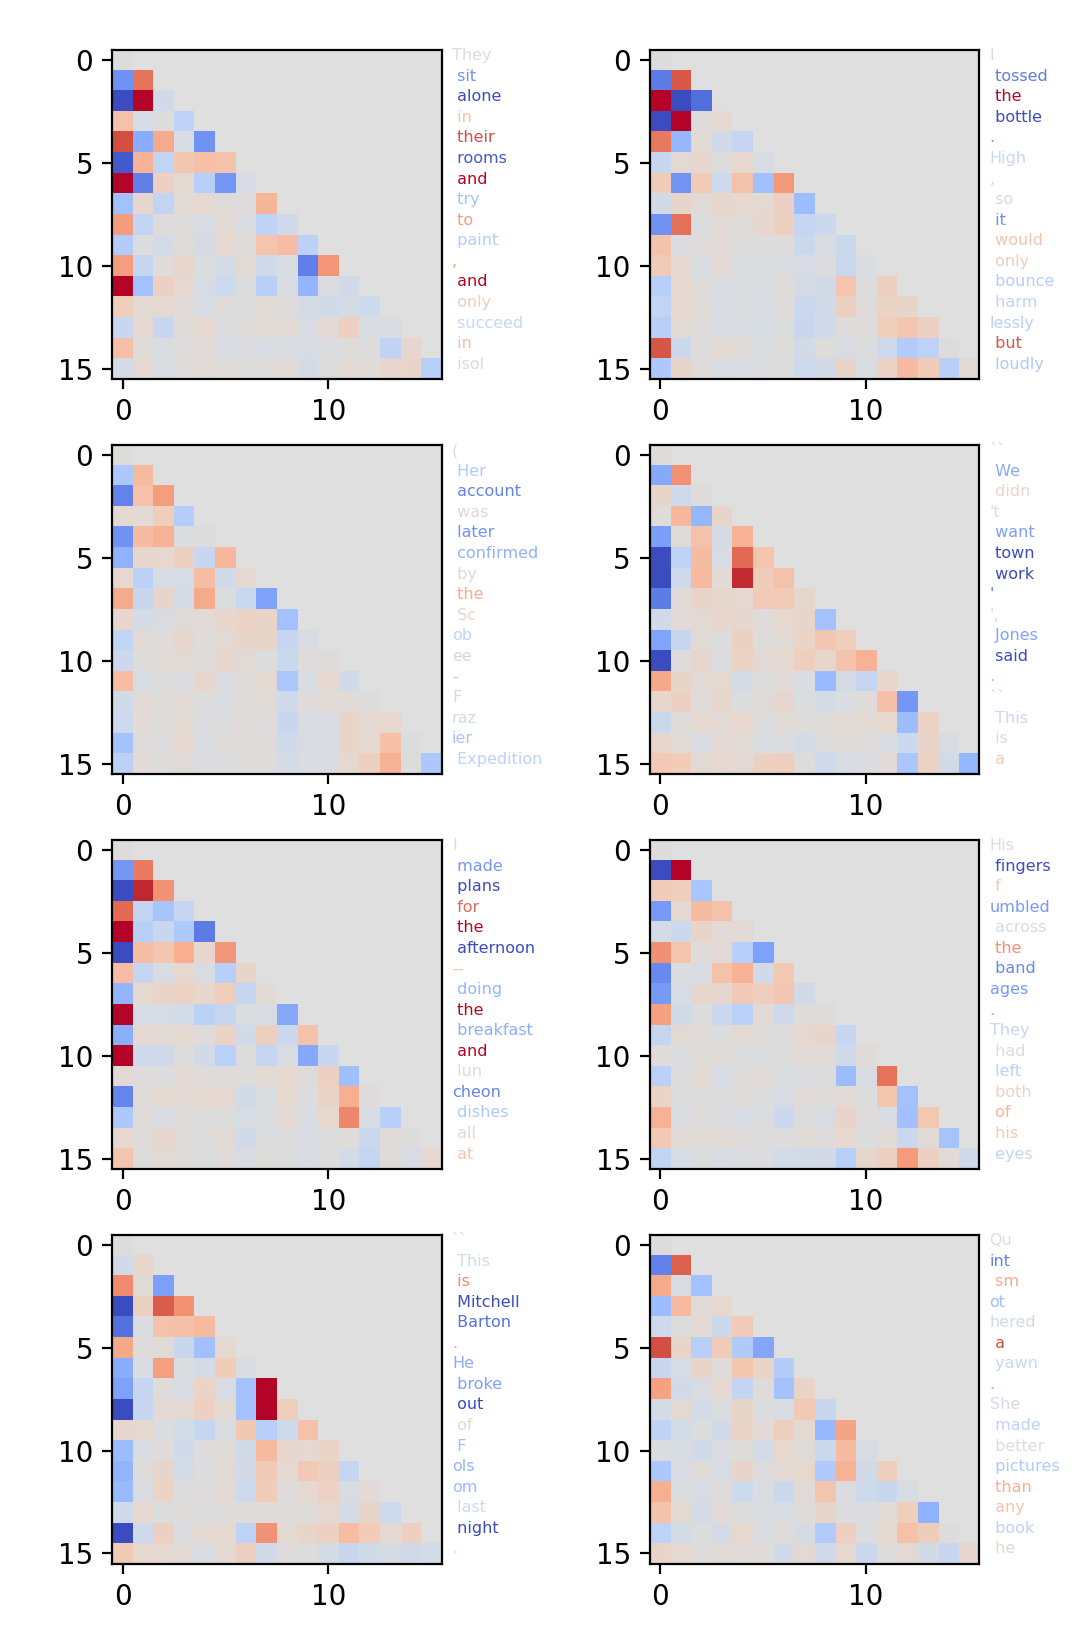
\includegraphics[width=\textwidth]{images/pca-component-2.png}
    \caption{Third PCA component annotated with prompt tokens}
    \label{fig:pca-component-2}
\end{figure}

\begin{figure}
    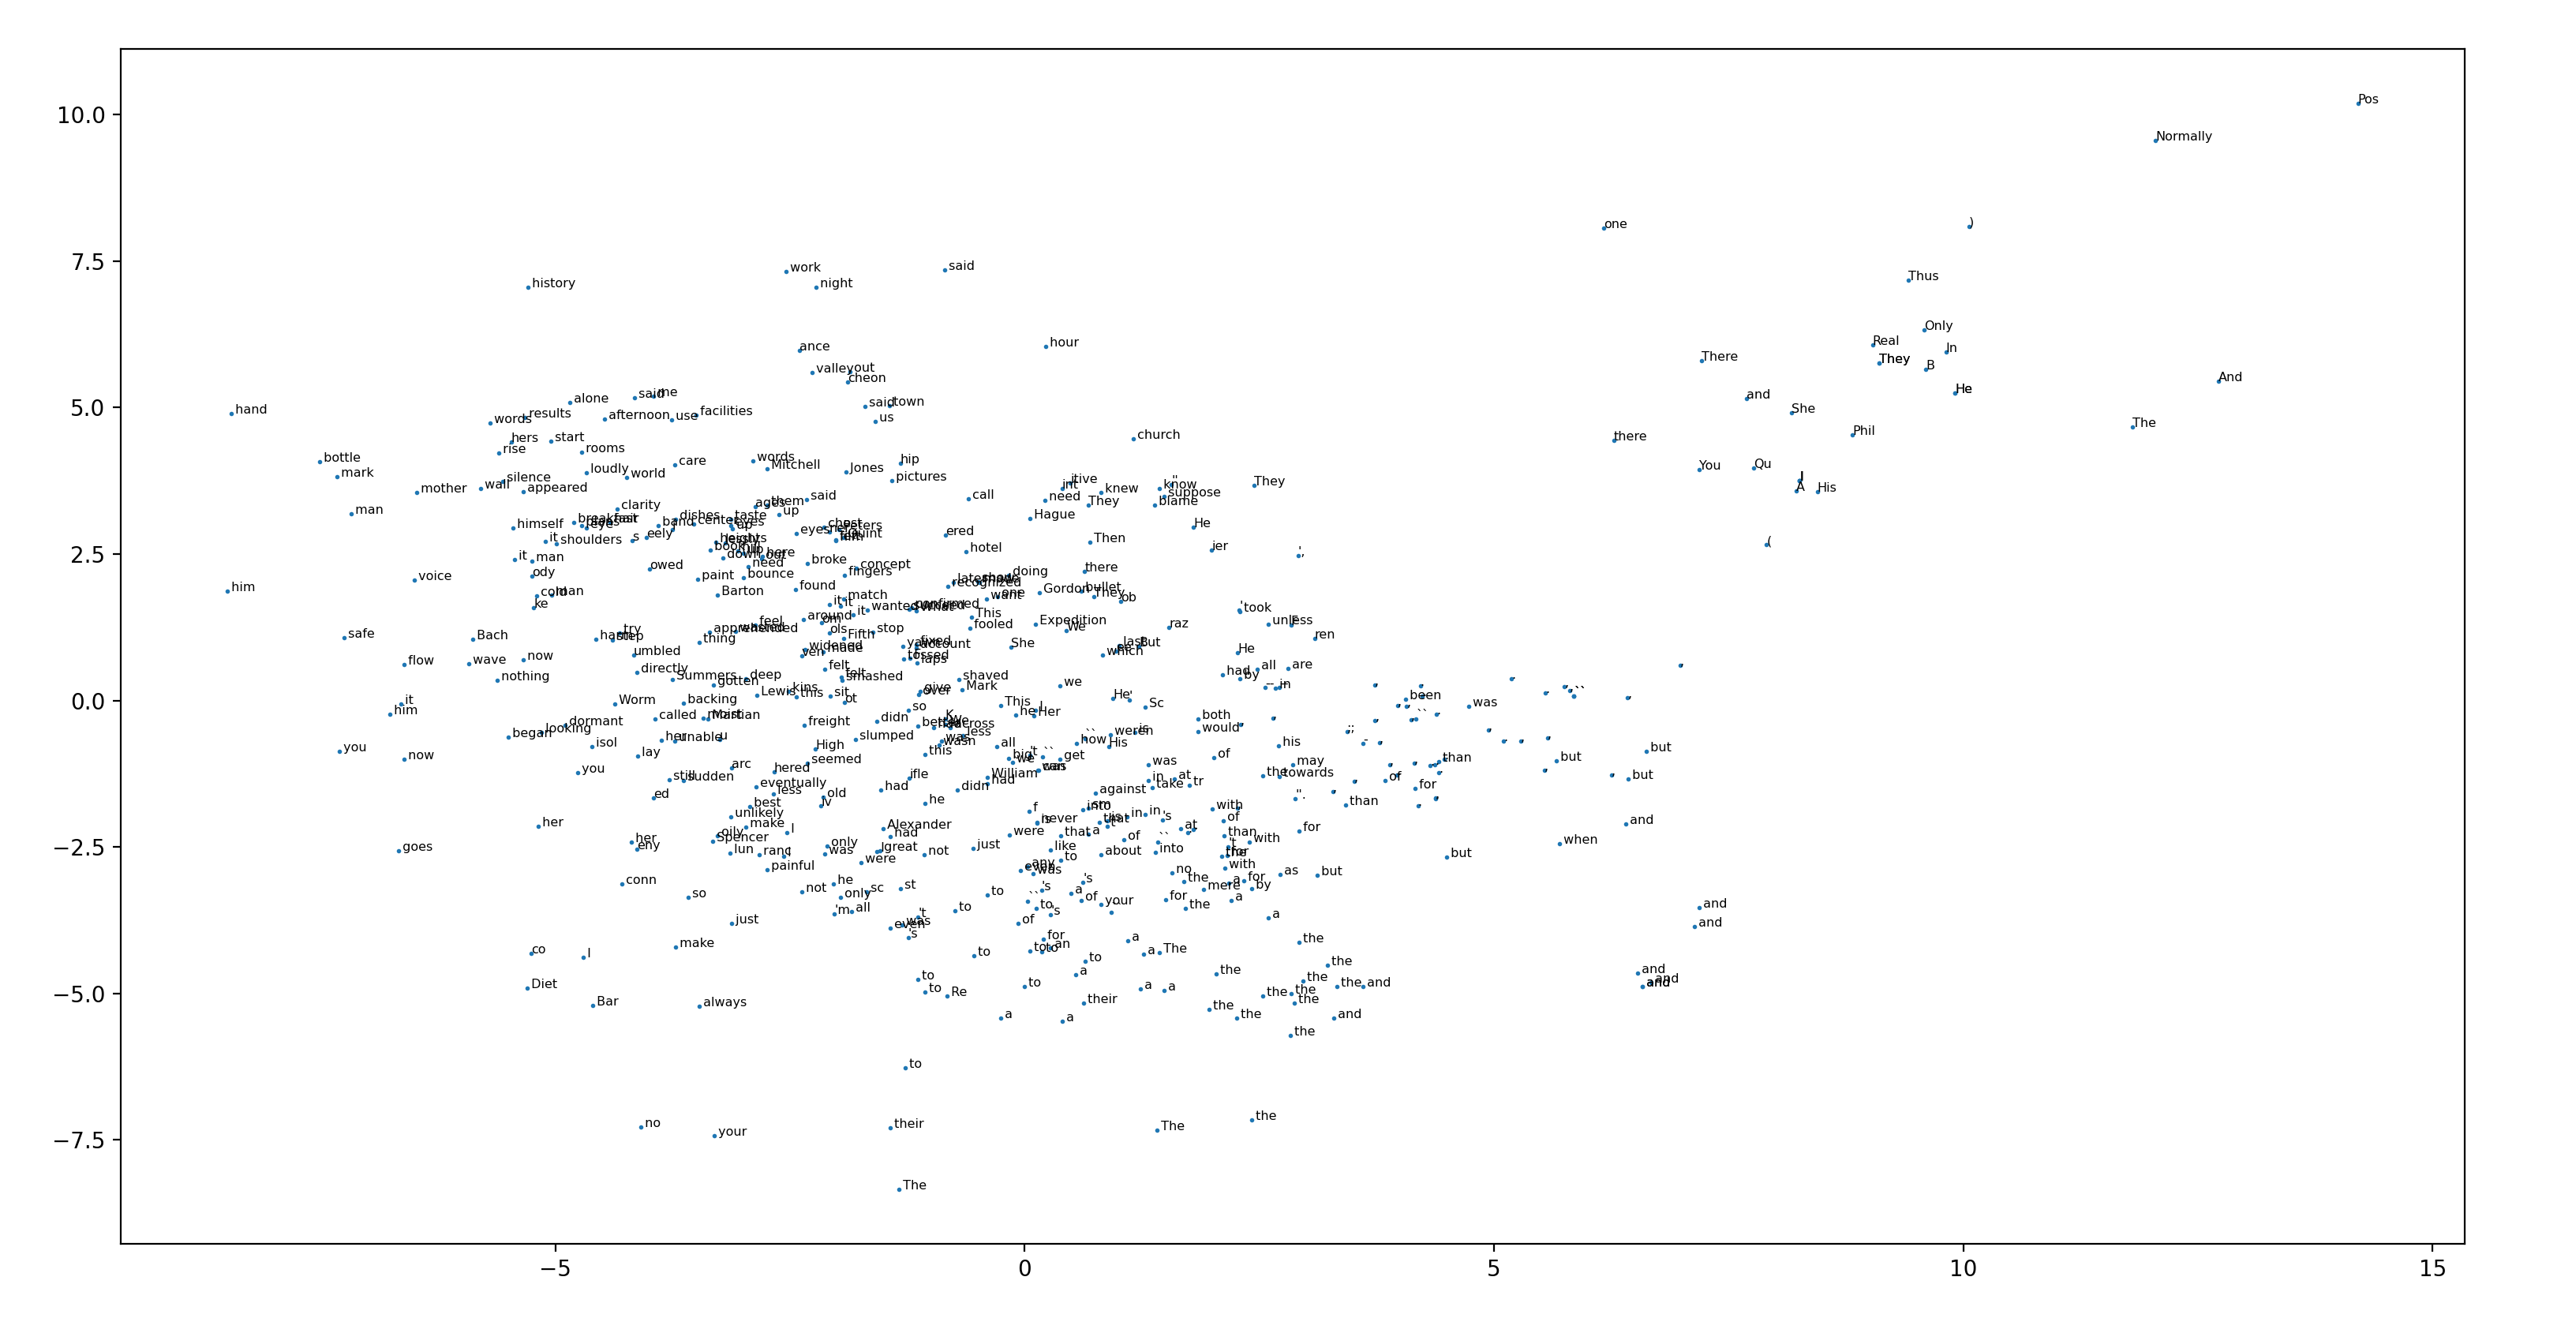
\includegraphics[width=\textwidth]{images/attending-to-first-token.png}
    \caption{PCA dimension reduction of how much each token attends to the first token in the prompt}
    \label{fig:attending-to-first-token}
\end{figure}

\subsection Knocking out heads

For the first prompt that we investigated, and for the first head of the first model, the clearest result came after 6 tokens. The prompt was "They sit alone in their rooms", and \ref{fig:knockout-one-prompt} shows that words such as "are", "were" and "will" are suppressed by the given head. Grammatically, the words should not be there (or are very unlikely), and the model has not fully learned this. However, the given head is in a sense "helping" the others out here.

In \ref{knockout-one-prompt-many-models} we extend this investigation to multiple models and heads - specifically everything in cluster 2. Some of the other models' heads seem to have a similar purpose, suppressing tokens such as "are" and "were". But not all of them.

Figure \ref{knockout-64prompt} shows how this effect extends across multiple prompts and all clusters. We see the turquoise cluster scattered across the bottom, the green cluster over to the left, and the peach/pink/gold clusters (which were near each other in the original plot) mixed together nearby. This suggests that for some clusters, there is a relatedness that goes beyond just similar attention patterns - they also have similar effects on the output.

\begin{figure}
	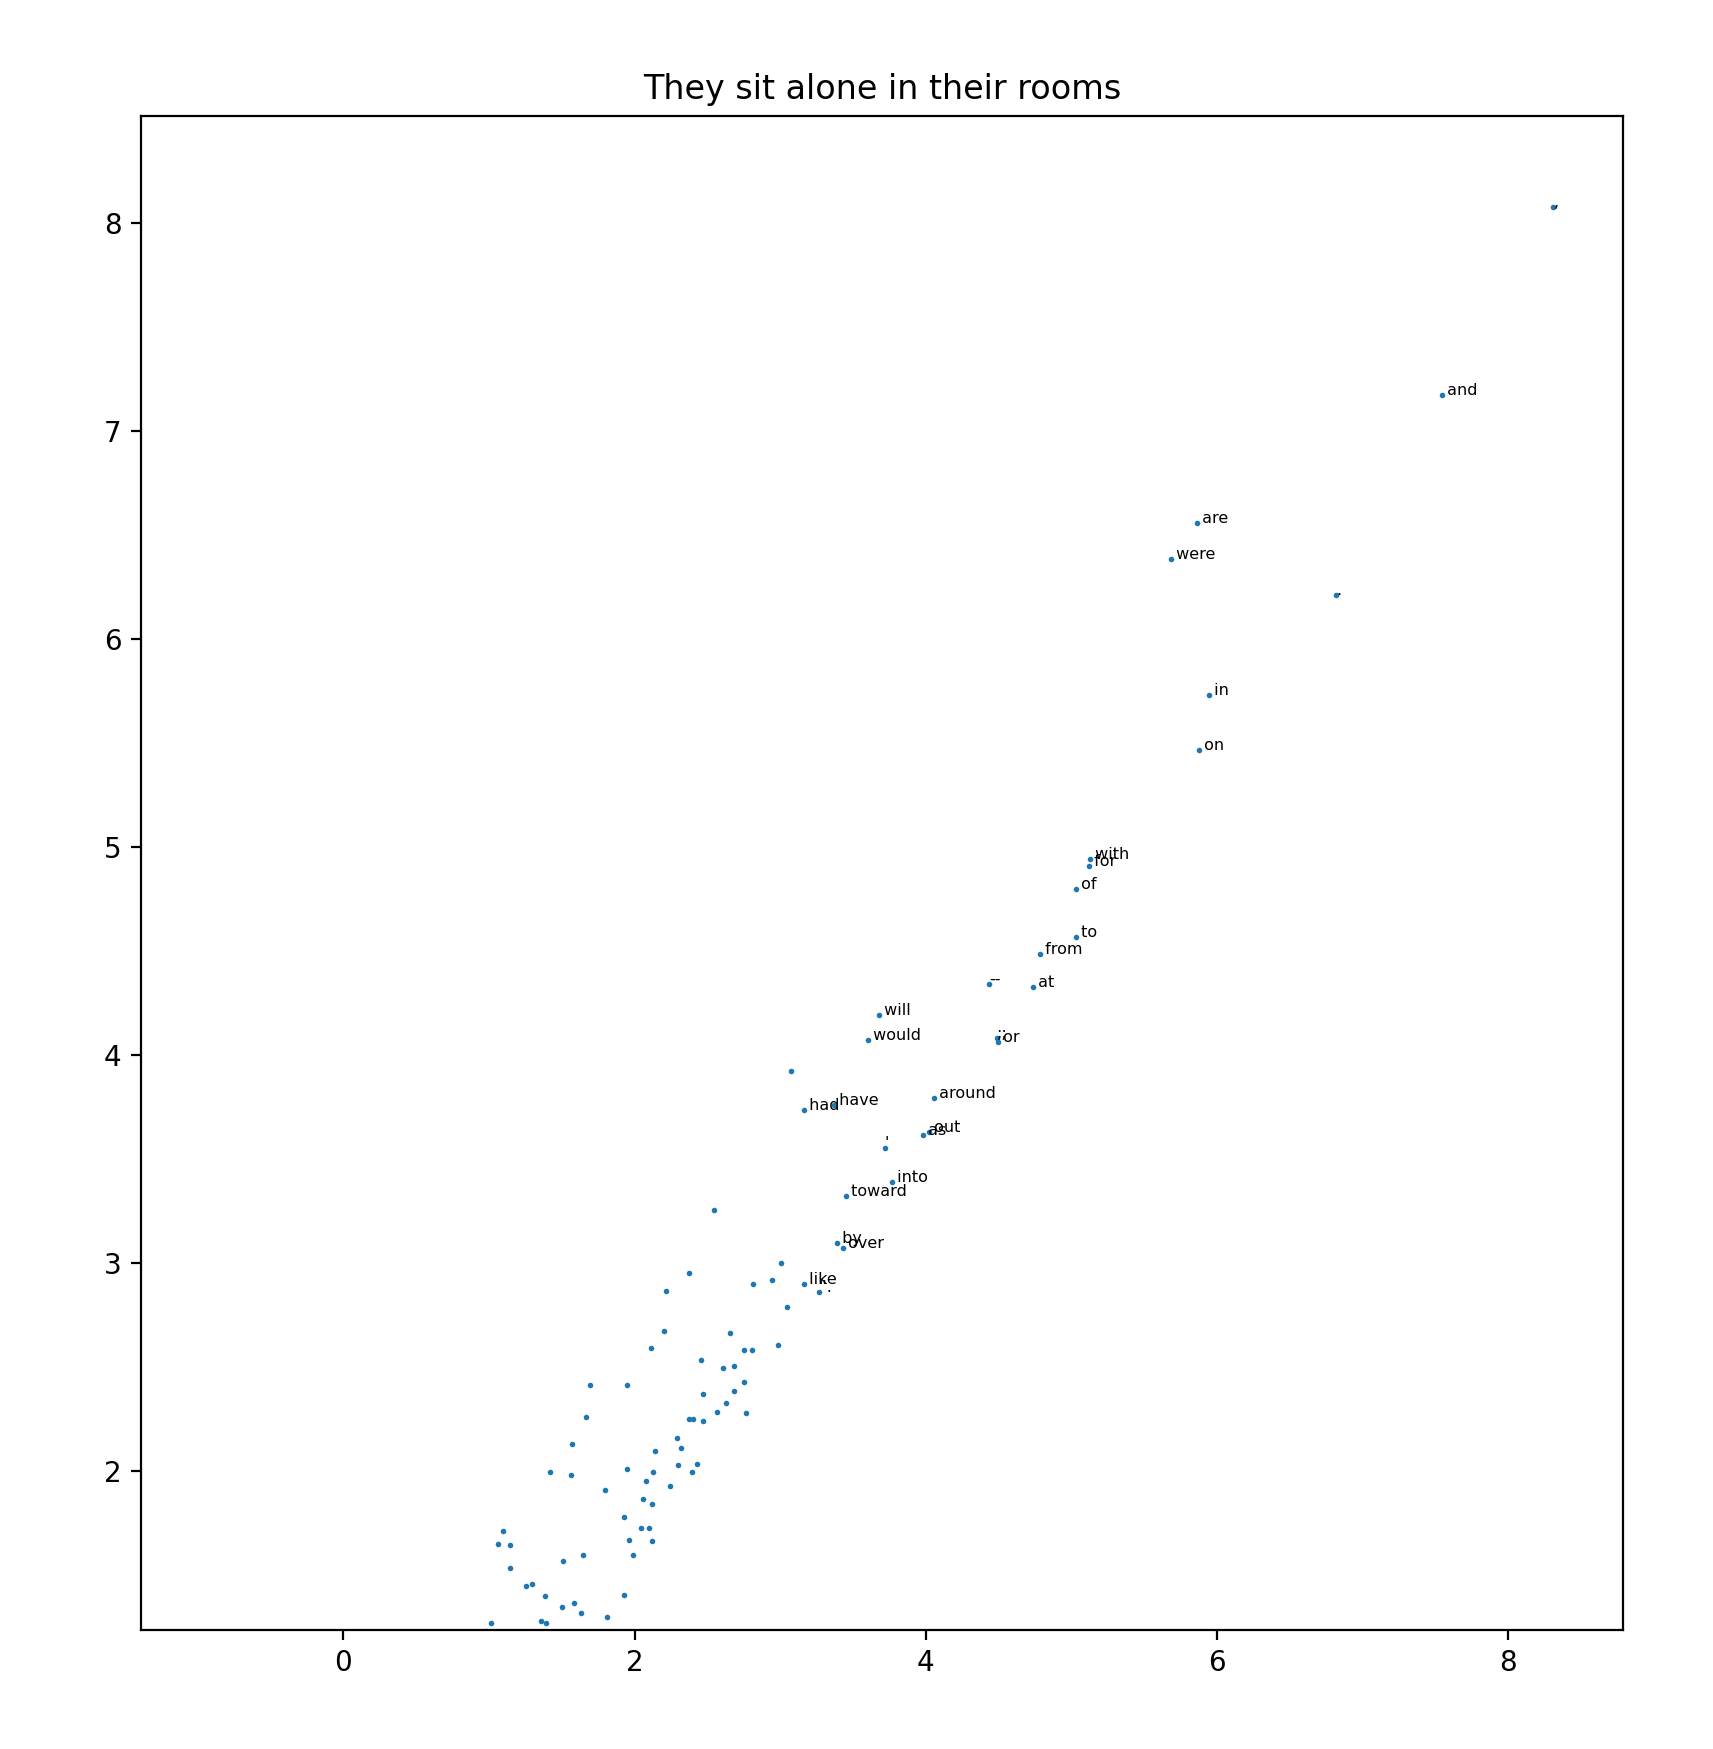
\includegraphics[width=\textwidth]{images/knockout-one-prompt.png}
	\caption{Scatterplot showing token logits emitted for the last token in the given prompt. X axis: original model. Y axis: model with head 1 knocked out.}
	\label{fig:knockout-one-prompt}
\end{figure}

\begin{figure}
	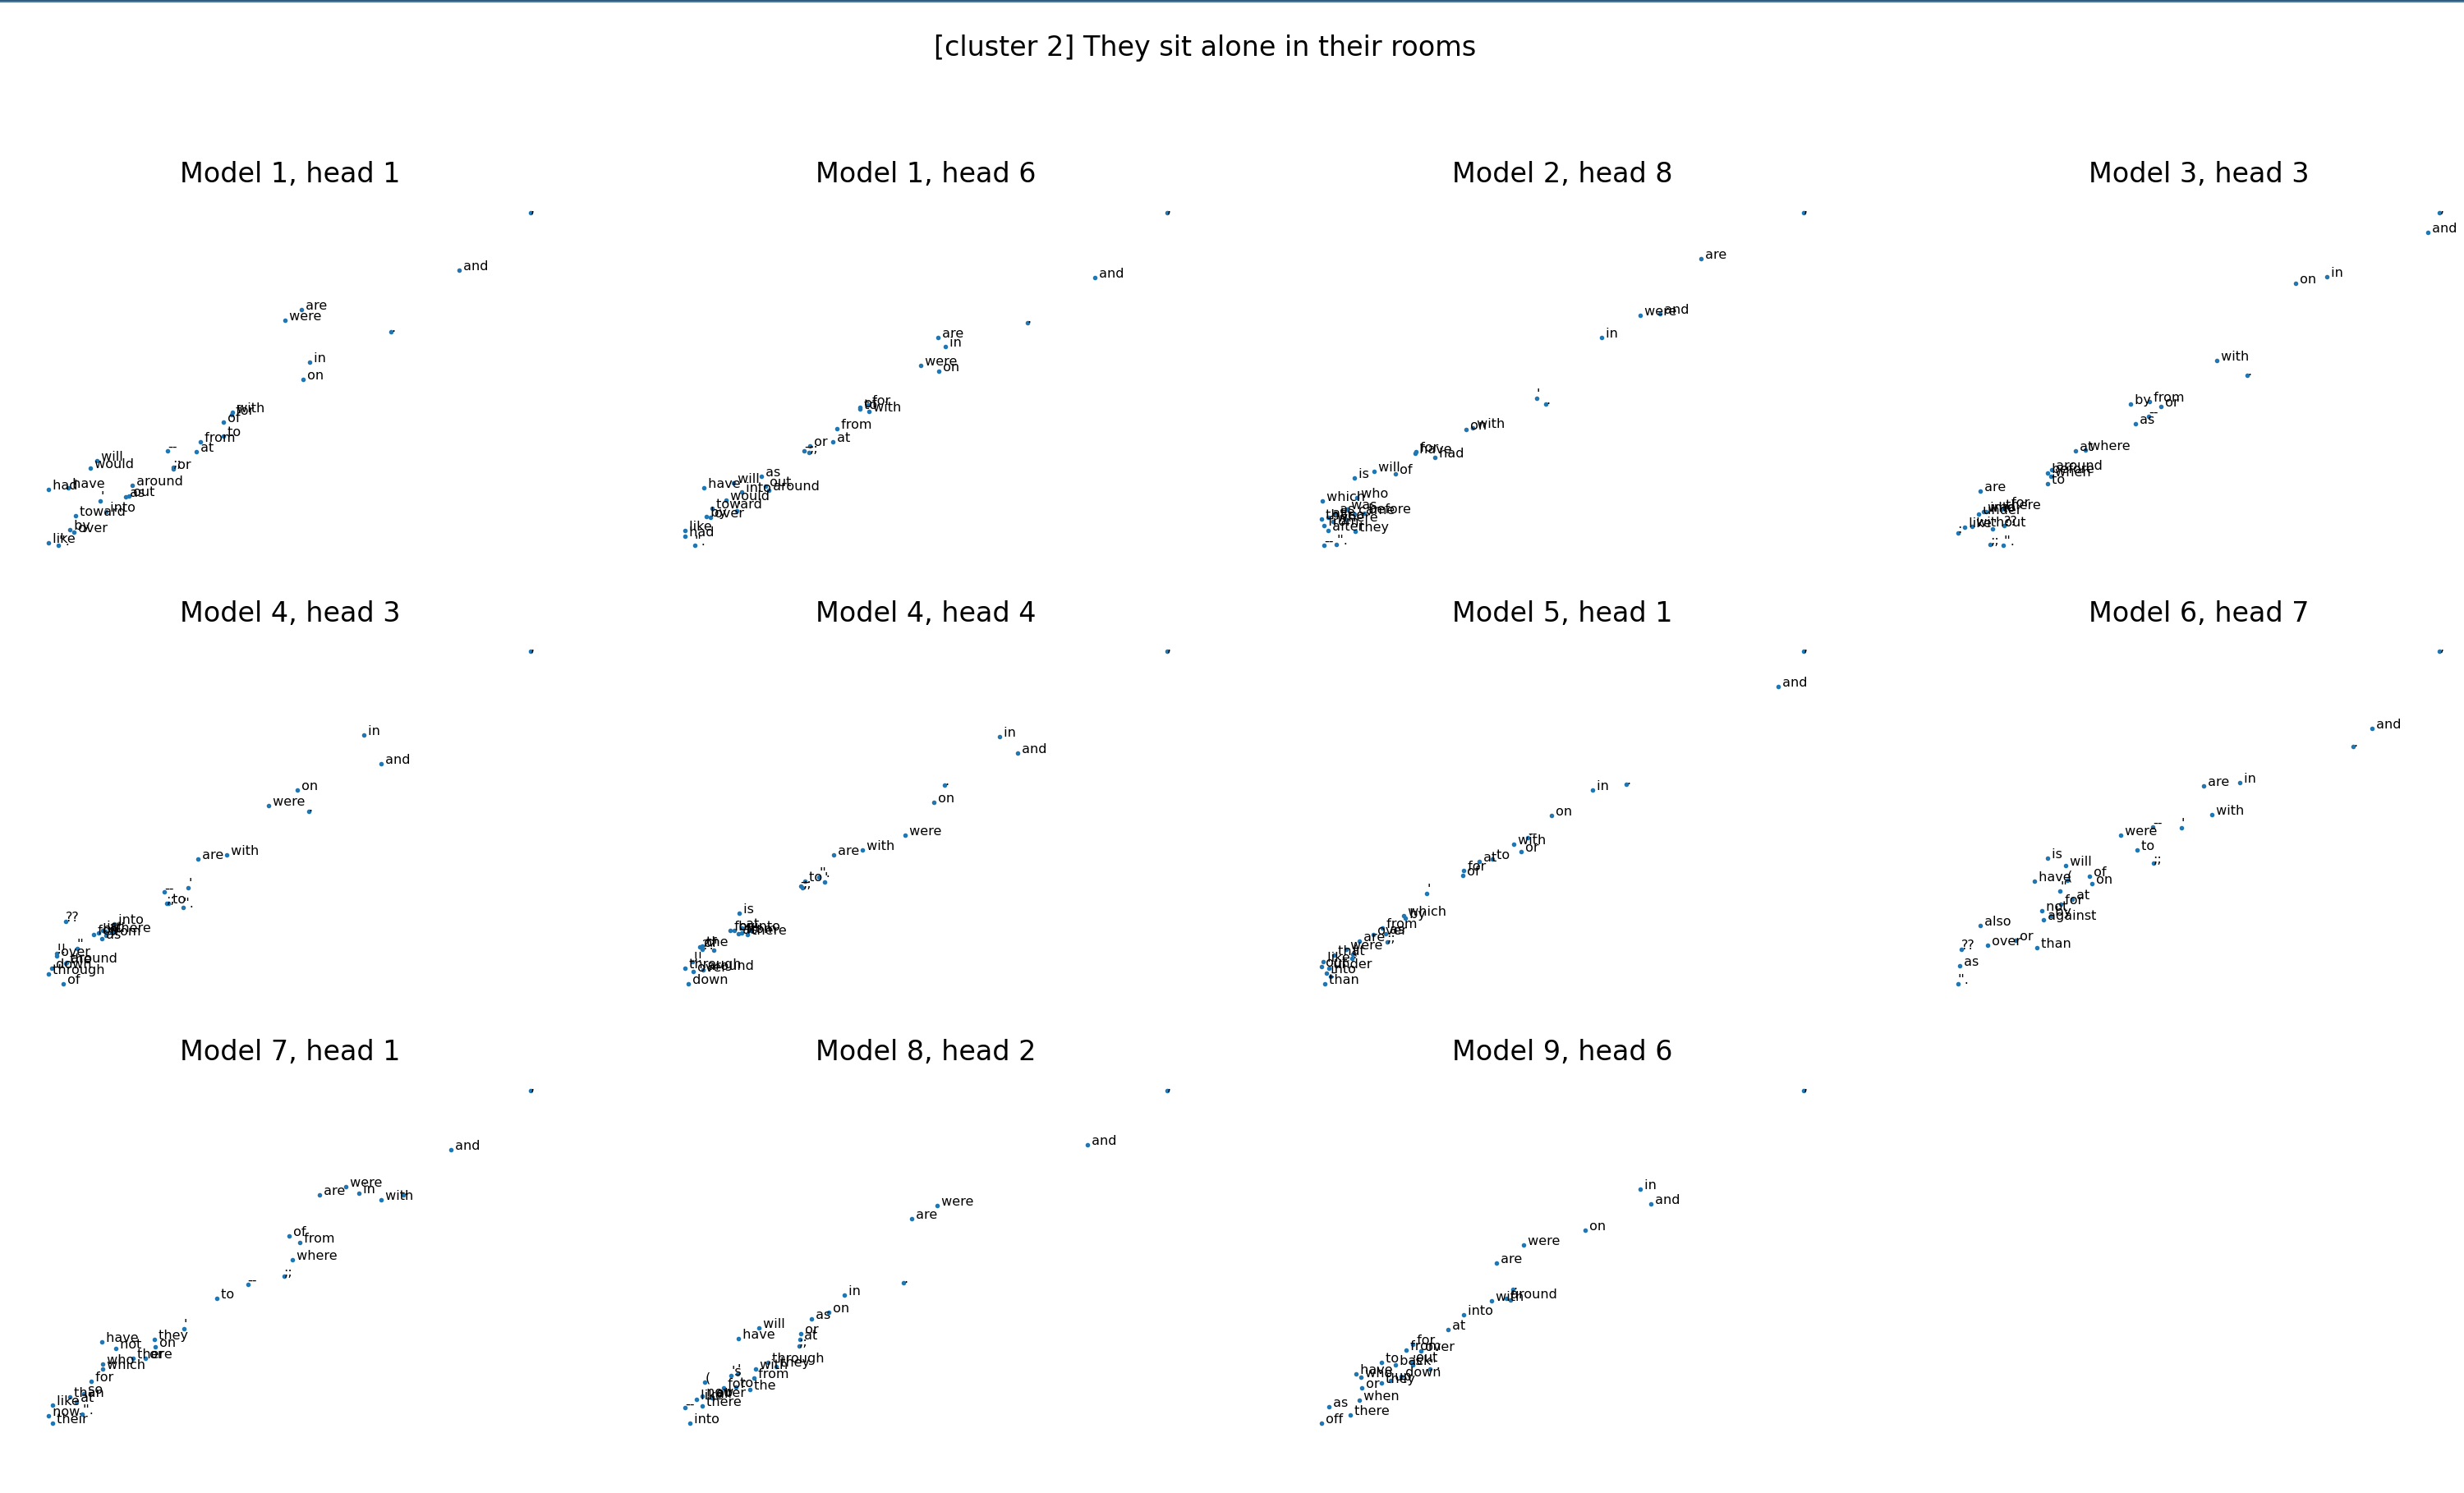
\includegraphics[width=\textwidth]{images/knockout-one-prompt-many-models.png}
	\caption{Scatterplot showing token logits emitted for the last token in the given prompt, for multiple models and heads in the same cluster. X axis: original model. Y axis: model with the given head knocked out.}
	\label{fig:knockout-one-prompt-many-models}
\end{figure}

\begin{figure}
	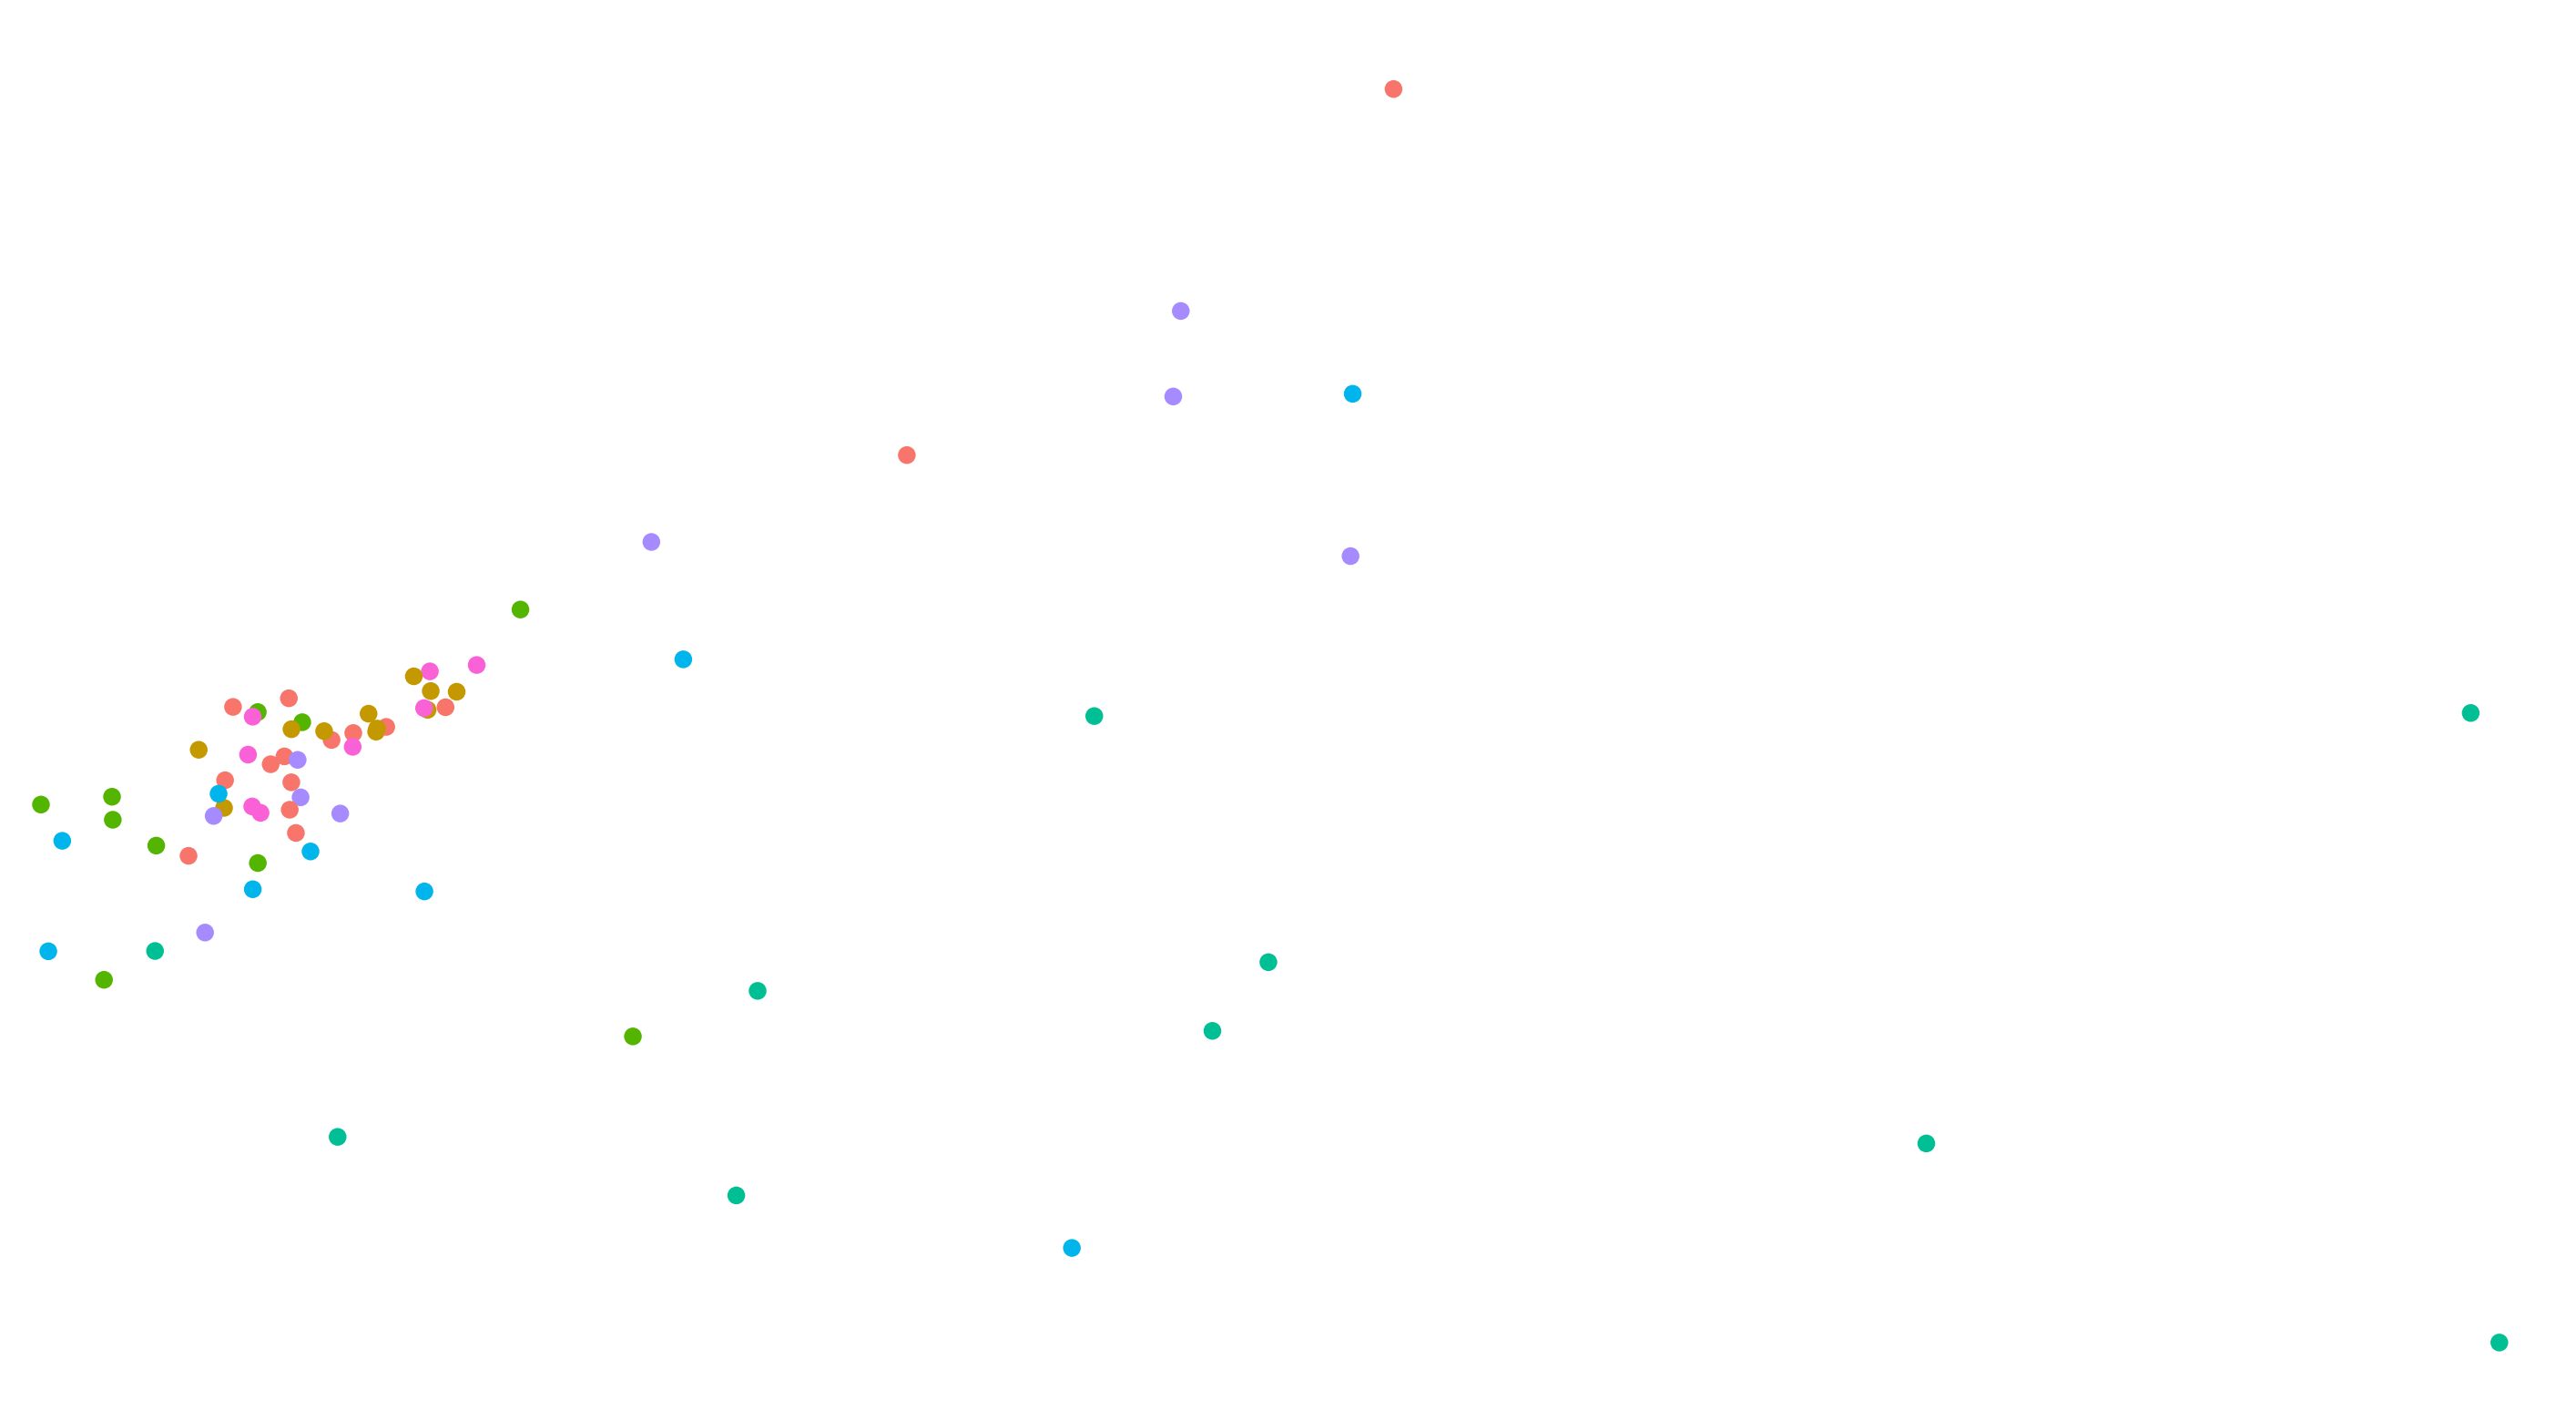
\includegraphics[width=\textwidth]{images/knockout-64prompt.png}
	\caption{PCA dimesnion reduction of model-heads, colored according to original clustering and positioned according to differences in probabilities when the given head is knocked out.}
	\label{fig:knockout-64prompt}
\end{figure}


\section{Discussion}


\label{sec:others}
\lipsum[8] \cite{kour2014real,kour2014fast} and see \cite{hadash2018estimate}.

The documentation for \verb+natbib+ may be found at
\begin{center}
  \url{http://mirrors.ctan.org/macros/latex/contrib/natbib/natnotes.pdf}
\end{center}
Of note is the command \verb+\citet+, which produces citations
appropriate for use in inline text.  For example,
\begin{verbatim}
   \citet{hasselmo} investigated\dots
\end{verbatim}
produces
\begin{quote}
  Hasselmo, et al.\ (1995) investigated\dots
\end{quote}

\begin{center}
  \url{https://www.ctan.org/pkg/booktabs}
\end{center}


\subsection{Figures}
\lipsum[10] 
See Figure \ref{fig:fig1}. Here is how you add footnotes. \footnote{Sample of the first footnote.}
\lipsum[11] 

\begin{figure}
  \centering
  \fbox{\rule[-.5cm]{4cm}{4cm} \rule[-.5cm]{4cm}{0cm}}
  \caption{Sample figure caption.}
  \label{fig:fig1}
\end{figure}

\begin{figure} % picture
    \centering
    \includegraphics{test.png}
\end{figure}

\subsection{Tables}
\lipsum[12]
See awesome Table~\ref{tab:table}.

\begin{table}
 \caption{Sample table title}
  \centering
  \begin{tabular}{lll}
    \toprule
    \multicolumn{2}{c}{Part}                   \\
    \cmidrule(r){1-2}
    Name     & Description     & Size ($\mu$m) \\
    \midrule
    Dendrite & Input terminal  & $\sim$100     \\
    Axon     & Output terminal & $\sim$10      \\
    Soma     & Cell body       & up to $10^6$  \\
    \bottomrule
  \end{tabular}
  \label{tab:table}
\end{table}

\subsection{Lists}
\begin{itemize}
\item Lorem ipsum dolor sit amet
\item consectetur adipiscing elit. 
\item Aliquam dignissim blandit est, in dictum tortor gravida eget. In ac rutrum magna.
\end{itemize}


\bibliographystyle{unsrt}  
%\bibliography{references}  %%% Remove comment to use the external .bib file (using bibtex).
%%% and comment out the ``thebibliography'' section.


%%% Comment out this section when you \bibliography{references} is enabled.
\begin{thebibliography}{1}

\bibitem{kour2014real}
George Kour and Raid Saabne.
\newblock Real-time segmentation of on-line handwritten arabic script.
\newblock In {\em Frontiers in Handwriting Recognition (ICFHR), 2014 14th
  International Conference on}, pages 417--422. IEEE, 2014.

\bibitem{kour2014fast}
George Kour and Raid Saabne.
\newblock Fast classification of handwritten on-line arabic characters.
\newblock In {\em Soft Computing and Pattern Recognition (SoCPaR), 2014 6th
  International Conference of}, pages 312--318. IEEE, 2014.

\bibitem{hadash2018estimate}
Guy Hadash, Einat Kermany, Boaz Carmeli, Ofer Lavi, George Kour, and Alon
  Jacovi.
\newblock Estimate and replace: A novel approach to integrating deep neural
  networks with existing applications.
\newblock {\em arXiv preprint arXiv:1804.09028}, 2018.

\end{thebibliography}


\end{document}


